\documentclass[dcc,sol]{fcfmcourse}
\usepackage{teoria}
\usepackage[utf8x]{inputenc}
\usepackage{amsmath}
\usepackage{amsfonts,setspace}
\usepackage{listings}
\usepackage{hyperref}
\usepackage{color}

\definecolor{pblue}{rgb}{0.13,0.13,1}
\definecolor{pgreen}{rgb}{0,0.5,0}
\definecolor{porange}{rgb}{0.9,0.5,0}
\definecolor{pgrey}{rgb}{0.46,0.45,0.48}

\lstset{language=Java,
  showspaces=false,
  showtabs=false,
  breaklines=true,
  showstringspaces=false,
  breakatwhitespace=true,
  commentstyle=\color{porange},
  keywordstyle=\color{pblue},
  stringstyle=\color{pgreen},
  basicstyle=\ttfamily,
  moredelim=[il][\textcolor{pgrey}]{$ $},
  moredelim=[is][\textcolor{pgrey}]{\%\%}{\%\%}
}

\newenvironment{codebox} {\small \ttfamily \obeylines \begingroup \setstretch{-2.4}} {\endgroup}

% COmpletar titulo
\title{Auxiliar 10 - Algoritmos de Ordenación}
\course[CC3001]{Algoritmos y Estructuras de Datos}
\professor{Nelson Baloian}
\professor{Patricio Poblete}
\assistant{Manuel Cáceres}
\assistant{Sebastián Ferrada}
\assistant{Sergio Peñafiel}

% Si pasas el comando usedate a la clase, la fecha aparecerá bajo la lista de auxiliares.
% Puedes usar el formato de fecha por defecto de latex (y traducirla usando babel)
% o puedes escribir lo que quieras con el comando \date.
% \date{1 de Septiembre, 2015}

%% En catedras se vio :
%% Quick Sort, dos formas, mediana de tres conjuntos chicos por inserción, solo un caso se ordena 
%%recursivamente la parte mas chica y la otra iterativa

%% Problemas propuestos en reunión:
%% - Programación de las maneras de quicksort, profiling de las version
%% - Merge Sort


\begin{document}
\maketitle

\vspace{-1ex}


\section*{Implementación de QuickSort}
\begin{problems}
\problem Asuma que tiene la función  \texttt{static int particionar(int[] a, int lo, int hi)} que escoge un pivote al azar del arreglo y lo particiona en dos mitades, una de los menores al pivote y otra de los mayores al pivote; la función retorna el índice en el que queda el pivote.\\
Utilizando lo anterior programe la función \texttt{static void quickSort(int[] a)} que ordena el arreglo con QuickSort.
\problem \subsection*{Particionar}
\begin{enumerate}

\item Programe la función particionar \footnote{Visualización y musicalización de este particionar en: \\ \href{https://0f1b206776b3b12da02dc4ce2b9f92f82512a815.googledrive.com/host/0B2GQktu-wcTicjRaRjV1NmRFN1U/index.html}{https://0f1b206776b3b12da02dc4ce2b9f92f82512a815.googledrive.com/host/0B2GQktu-wcTicjRaRjV1NmRFN1U/index.html}} según el invariante :
\begin{center}
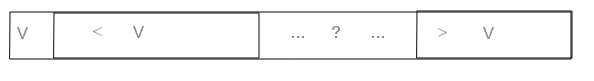
\includegraphics[scale=0.5]{imagenes/particionar1.png}
\end{center}

\item Programe la función particionar según el invariante :
\begin{center}
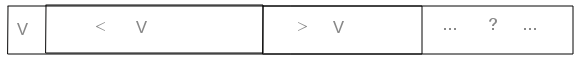
\includegraphics[scale=0.5]{imagenes/particionar2.png}
\end{center}


\item Programe la función particionar según el invariante :
\begin{center}
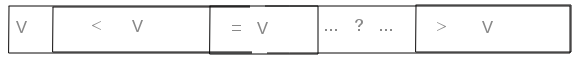
\includegraphics[scale=0.5]{imagenes/particionar3.png}
\end{center}
\end{enumerate}
\end{problems}
\newpage
\section*{Seleccionar}
\begin{problems}
\problem El problema de ``seleccionar'' el elemento $k$ de un arreglo $a$ consiste en encontrar $a[i]$ tal que existen $k-1$ elementos menores a este en el arreglo.
\begin{enumerate} [a)]
    \item Programe función \texttt{static int seleccionar(int[] a, int k)} que selecciona el elemento $k$ del arreglo $a$. Su función debe tener un número de comparaciones de $\Theta (n \log n)$.
    \item Reescriba la función anterior de manera que tenga un caso promedio de $\mathcal{O}(n)$.
    \\ \textbf{Hint:} Utilice la función particionar. ¿De que orden es el peor caso de este algoritmo? ¿Es conveniente usarlo en la práctica?.
\end{enumerate}

\end{problems}



\end{document}